% !TEX encoding = UTF-8

\documentclass{article}
\usepackage{luatexja-fontspec}
\setmainjfont{SimSun}

\usepackage[T1]{fontenc}
\usepackage{beramono}
\usepackage{booktabs}
\usepackage{listings}
\usepackage{xcolor}

\title{gSpan算法实现报告}
\author{郑淇木  1501214427}
\date{\today}

\usepackage{xcolor}

\definecolor{dkgreen}{rgb}{0,0.6,0}
\definecolor{gray}{rgb}{0.5,0.5,0.5}
\definecolor{mauve}{rgb}{0.58,0,0.82}

\lstdefinestyle{mStyle}{
  frame=tb,
  language=scala,
  aboveskip=3mm,
  belowskip=3mm,
  showstringspaces=false,
  columns=flexible,
  basicstyle={\small\ttfamily},
  %numbers=none,
  numbers=left,
  numbersep=5pt,
  numberstyle=\tiny\color{gray},
  keywordstyle=\color{blue},
  commentstyle=\color{dkgreen},
  stringstyle=\color{mauve},
  frame=single,
  breaklines=true,
  breakatwhitespace=true,
  tabsize=2,
}

\begin{document}
\maketitle

\begin{abstract}
在本次课程作业中,我使用Scala语言对频繁子图挖掘算法gSpan进行了实现,对算法中的关键步骤进行并行优化以提高执行效率,并将程序所得输入与论文作者所给出程序的输出进行比对确认了算法实现的正确性。

\end{abstract}


\section{Introduction}
本次作业的主要内容是理解并实现频繁子图挖掘中的gSpan算法\cite{gspan2002,gspanlong}。
gSpan算法所面向的问题是对一个有点label、边label的图集合,从中挖掘频繁子图。gSpan的核心是给出了对任意的图的唯一最小编码,并在此基础上把频繁子图挖掘问题转化为深度优先搜索问题。除此之外,算法根据最小编码的性质对搜索空间进行了有效剪枝,有效降低了算法的复杂度。

在本项目中,我使用了Scala语言完成了gSpan算法的实现,并将所得输出与论文作者所给出程序的输出进行比对,确认了代码运行结果的正确性。
本报告将对算法的实现方式、所使用数据结果等方面进行介绍。其中Section 2介绍了算法实现的表现,Section 3介绍了算法所使用的数据结构,Section 4、Section 5介绍了算法的框架及一些值得注意的细节,Section 6介绍了对算法的并行化。

项目地址: https://github.com/zhengqm/gSpan-Scala

\section{Performance and Result}

我基于不同support level对所给数据集进行挖掘,所得结果、程序在笔记本上的运行时间(三次平均)如下所示:

\vspace{0.3cm}
\begin{tabular}{rrrr}
\toprule
 Support threshold&  Runtime(sec) &  \#Freq graphs &  \#Freq graphs(at least 1 edge) \\
\midrule
    0.01 &       523.3 &            59129 &                              59120 \\
    0.05 &        54.2 &             1838 &                               1832 \\
    0.10 &        27.7 &              460 &                                455 \\
    0.15 &        22.5 &              225 &                                220 \\
    0.20 &        19.2 &              126 &                                122 \\
    0.25 &        14.7 &               86 &                                 82 \\
    0.30 &        12.8 &               55 &                                 52 \\
\bottomrule
\end{tabular}
\vspace{0.3cm}

其中,运行时间随support level的变化趋势如下所示:

\begin{figure}
  \centering

  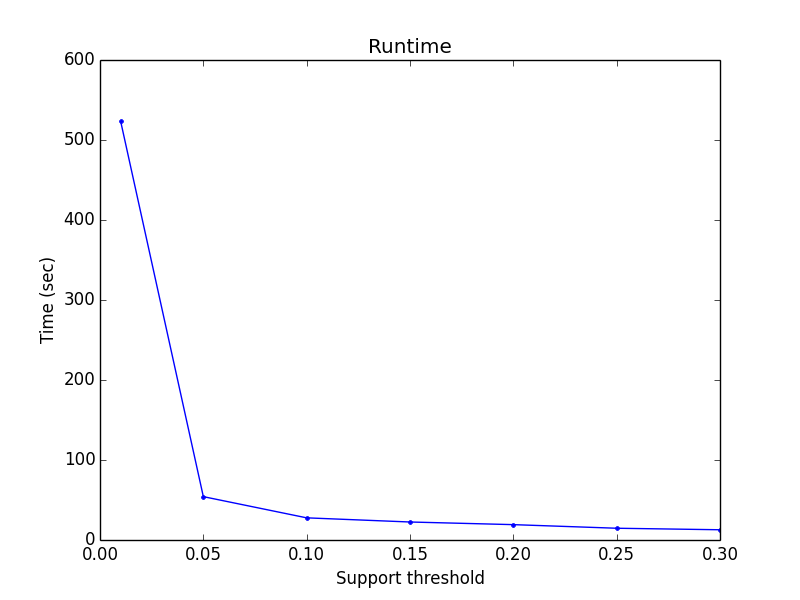
\includegraphics[width=0.6\textwidth]{time.png} 
\end{figure}


\section{Data Structure}

项目所定义的数据结构主要包含两部分,图存储相关的数据结构及算法运行相关的数据结构,其中图存储相关的数据结构在Section3.1中介绍,算法运行相关的数据结构在Section3.2中介绍。

\subsection{Edge, Vertex, Graph and GraphSet}

图存储相关的数据结构主要包含边、点、图及图集合,具体定义如下:
\begin{lstlisting}[style=mStyle]

class Edge(val fromId: Int, 
            val toId: Int, 
            val fromLabel: Int, 
            val edgeLabel: Int, 
            val toLabel: Int) {
}

class Vertex(val id: Int, 
              val label: Int, 
              var edges: List[Edge]) {
 }

class Graph(val id: Int, val vertices: IndexedSeq[Vertex]) {

  val innerLookup: Map[Int, Vertex] = vertices.map { vertex => (vertex.id, vertex)}.toMap

  def findVertex(vertexId: Int): Vertex = {
    innerLookup(vertexId)
  }
}

class GraphSet(val graphSet: IndexedSeq[Graph])
\end{lstlisting}

其中Edge、Vertex、GraphSet是对数据的简单封装,Graph除了对边进行封装外,还根据算法的需求增加了一个Vertex ID至Vertex对象的Map数据结构以加速对节点的获取。



\subsection{EdgeCode, DFSCode and FinalDFSCode}

算法运行相关的数据结构主要包括子图边的存储结构、子图编码的存储结构:

\begin{lstlisting}[style=mStyle]
class EdgeCode( val fromId: Int, 
                val toId: Int, 
                val fromLabel: Int, 
                val edgeLabel: Int, 
                val toLabel: Int) {
  def toTuple = (fromId, toId, fromLabel, edgeLabel, toLabel)
}

class DFSCode(val codes: IndexedSeq[EdgeCode], 
              val graphSet: List[(Int, Map[Int, Int])], 
              val support: Int) {
}

class FinalDFSCode(codes: IndexedSeq[EdgeCode], support: Int) {
}

\end{lstlisting}

其中EdgeCode是对数据的简单封装,结构与Edge数据结构相同,使用不同的类存储相同的数据结构是为了更好地利用类型系统保证程序的正确性。
DFSCode数据结构记录了子图的结构,包含了边的序列(codes),与原图节点的对应(graphSet)及其支撑数量(support)。
FinalDFSCode数据结构用于存储所得到的频繁子图,与DFSCode相比删除了对与原图节点的对应的信息的存储。

\section{Basic Ideas}
本项目根据论文中作者给出的框架对算法进行了实现,具体来说:

\begin{lstlisting}[style=mStyle]
def main(args: Array[String]) {
  // ... code for setup ...
  val (gs, vertexLabelCounter, edgeLabelCounter) = loadDataFileAndCount("graph.data")
  val s = new ListBuffer[FinalDFSCode]

  var (graphSet, s1) = removeInfrequentVerticesAndEdges(gs, minSupport, vertexLabelCounter, edgeLabelCounter)

  for (edgeCode <- s1) {
    val dfsGraphSet = projectWithOneEdge(graphSet, edgeCode)
    val support = dfsGraphSet.map(_._1).distinct.size
    val dfsCode = new DFSCode(IndexedSeq(edgeCode), dfsGraphSet, support)
    subgraphMining(graphSet, s, dfsCode, minSupport)
    graphSet = shrink(graphSet, edgeCode)
  }
  // ... code for output ...
}
\end{lstlisting}

项目的主函数可以与原文给出的伪代码进行一一对应。
其中Line 3完成了对数据文件的读取,建立图数据结构并对点、边的label进行了计数。
Line 4新建了用于存储最终结果的数据结构,对应于原文伪代码中的S变量。
Line 6根据label的计数结果,对图集合进行重建,并返回频发的边集合,对应于原文伪代码中的S1变量。
在此之后,Line 8 至 Line 14则对于S1中的所有边,在图集合中进行投影,并在投影所得图集上进行搜索,在搜索结束后从图集合中将其删除并进入下一次迭代。

此外,算法的主体subgraphMining的实现如下:
\begin{lstlisting}[style=mStyle]
def subgraphMining(graphSet: GraphSet, 
                   s: ListBuffer[FinalDFSCode], 
                   dfsCode: DFSCode, 
                   minSupport: Int): Unit = {

  if (isMinDFSCode(dfsCode)) {
    val support = dfsCode.support
    if (support >= minSupport) {

      s += new FinalDFSCode(dfsCode.codes, support)
      val (childrenGraphSet, childrenCounting) = enumerateSubGraph(graphSet, dfsCode)
      val supportedChild = childrenCounting
                  .filter(_._2 >= minSupport)
                  .keys
                  .toList
                  .sortWith((e1, e2) => edgeCodeCompare(e1, e2) < 0)

      for(child <- supportedChild) {
        val edgeCode = new EdgeCode(child._1,child._2,child._3,child._4,child._5)
        val codes = dfsCode.codes :+ edgeCode
        val projectedGraphSet = childrenGraphSet.get(child).get.toList
        val extendedDFSCode = new DFSCode(codes, projectedGraphSet, childrenCounting.get(child).get)
        subgraphMining(graphSet, s, extendedDFSCode, minSupport)
      }
    }
  }
}
\end{lstlisting}

在对编码完成最小编码判定(Line 6)及最小支撑判定(Line 8)之后,算法将该编码加入结果列表之中(Line 10),枚举从该子图可能产生的增长边并统计其支撑数(Line 11)。在此之后对所得的增长边根据最小支撑要求进行筛选并进行排序(Line 12 to 16)。
最后对符合要求的增长边建立图数据结构,并对算法进行递归调用。

\section{Interesting Details}

\subsection{Check for minimal DFS codes}

在进行子图挖掘前,一个有效的剪枝策略是将不满足最小DFS Codes要求的子图删除,这需要程序完成对最小DFS Codes的判定。一个简单但低效的做法是对于任意子图,产生其所有的DFS codes,从中选取最小的code并进行比较,这一做法相当于枚举一张图的所有表示方法并在最后进行比较。

而实际上,在对codes进行判定时,并不需要实际产生完整的codes序列,而是可以使用较为启发式的方法对图进行“增量验证”。具体来说,算法可以从图中不同的点开始进行搜索,在每一步依据排序规则逐步产生最小序列,将所得到的code与输入的code进行增量比较,若所得到的code较大,则可停止进一步搜索;若所得到的code较小,则函数应返回False;若二者相等,则可以继续产生codes并继续比较。这一做法,相比简单的先产生后比较,效率存在明显提升。

\subsection{Pruning of Invalid Children}

\subsubsection{Forward Growth}

对于最右路径上的增长,设增长节点为v且v不是最右节点,则从v增长的边须大于等于最右路径中v的增长边(否则将违反最小DFS codes的要求)。

\subsubsection{Backward Growth}

对于最右路径上的增长,设增长节点为v,目标节点为w。则新增长的边须大于等于最右路径中w的增长边(否则将违反最小DFS codes的要求)。
此外,若原图中已有从v增长的反向边,则新增长的边须大于等于所有由v增长的反向边(否则将导致重复)。

\section{Parallel Execution}

在完成算法的实现后,我对程序进行了profile以确定速度瓶颈并进行优化。Profile的结果显示程序中耗时最多的步骤是算法中的enumerate步骤,即对给定子图在支撑它的图中搜索其增加一条边的频繁子图。考虑到在枚举新增一条边的子图时,对支撑该子图的graphSet的搜索可以并行执行,遂对该步骤进行并行优化。

具体而言,在enumerate函数中,程序定义了一个帮助函数对给定子图、映射进行搜索:
\begin{lstlisting}[style=mStyle]
def aux(graphId: Int, mapping: Map[Int, Int], rightMostPath:IndexedSeq[Int]) = {
  val graph = graphSet.graphSet(graphId)
  val backwardGrowth = findBackwardGrowth(graph, mapping, dfsCode, rightMostPath)
  val forwardGrowth = findForwardGrowth(graph, mapping, dfsCode, rightMostPath)
  (graphId, forwardGrowth, backwardGrowth)
}
\end{lstlisting}

在此基础上,对于支撑该子图的graphSet,利用Scala collections提供的并行功能,并行调用上述函数:

\begin{lstlisting}[style=mStyle]
val pGraphSet = dfsCode.graphSet.par
val result  = pGraphSet.map(gs => aux(gs._1, gs._2, rightMostPath)).toList
\end{lstlisting}

其中 Line 1 把graphSet变换位支持并行操作的collection,Line 2则对该collection进行map操作,即并行的对collection中的每个元素调用帮助函数,并将返回结果存储在一个列表中。

在完成上述优化后,对子图后续children的枚举被分散到多核中并行执行,程序的CPU占用率保持在400\%至700\%之间,程序运行时间显著减少,运行效率得到了显著提升。


\begin{thebibliography}{9}

\bibitem{gspan2002}
  Xifeng Yan and Jiawei Han. 2002. \emph{gSpan: Graph-Based Substructure Pattern Mining}. In Proceedings of the 2002 IEEE International Conference on Data Mining (ICDM '02). IEEE Computer Society, Washington, DC, USA, 721-.


\bibitem{gspanlong}
  Xifeng Yan and Jiawei Han. 2002. \emph{gSpan: Graph-Based Substructure Pattern Mining}. UIUC Technical Report, UIUCDCS-R-2002-2296

\end{thebibliography}

\end{document}